% Generated by code/ch12_grape.py -- do not edit by hand.
\definecolor{qocA}{rgb}{0.00,0.45,0.70}
\definecolor{qocB}{rgb}{0.90,0.60,0.00}
\definecolor{qocC}{rgb}{0.00,0.62,0.45}
\definecolor{qocD}{rgb}{0.80,0.40,0.00}
\definecolor{qocE}{rgb}{0.80,0.60,0.70}
\definecolor{qocF}{rgb}{0.35,0.70,0.90}
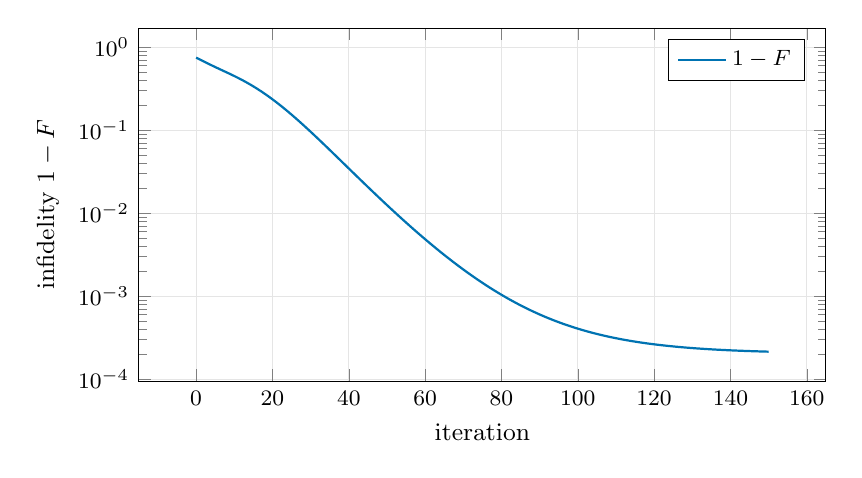
\begin{tikzpicture}[]
\begin{axis}[width=0.85\linewidth, height=0.5\linewidth, xlabel={iteration}, ylabel={infidelity $1-F$}, legend pos=north east, legend style={font=\footnotesize}, tick label style={font=\footnotesize}, label style={font=\small}, grid=major, grid style={gray!20}, ymode=log]
\addplot[thick, qocA] coordinates {(0,0.75104) (1,0.71314) (2,0.67628) (3,0.64137) (4,0.6088) (5,0.57859) (6,0.55046) (7,0.52402) (8,0.49886) (9,0.4746) (10,0.45098) (11,0.4278) (12,0.40495) (13,0.3824) (14,0.36014) (15,0.33822) (16,0.31672) (17,0.29571) (18,0.27528) (19,0.25551) (20,0.23649) (21,0.21828) (22,0.20095) (23,0.18454) (24,0.16907) (25,0.15456) (26,0.14101) (27,0.12842) (28,0.11676) (29,0.106) (30,0.096109) (31,0.087041) (32,0.078752) (33,0.071194) (34,0.064317) (35,0.058072) (36,0.052412) (37,0.04729) (38,0.042659) (39,0.038479) (40,0.034708) (41,0.031309) (42,0.028248) (43,0.025493) (44,0.023013) (45,0.020783) (46,0.018777) (47,0.016973) (48,0.015351) (49,0.013892) (50,0.012579) (51,0.011399) (52,0.010337) (53,0.0093813) (54,0.0085208) (55,0.007746) (56,0.0070479) (57,0.0064187) (58,0.0058514) (59,0.0053396) (60,0.0048777) (61,0.0044605) (62,0.0040836) (63,0.0037428) (64,0.0034345) (65,0.0031554) (66,0.0029026) (67,0.0026735) (68,0.0024657) (69,0.0022771) (70,0.0021058) (71,0.0019501) (72,0.0018085) (73,0.0016796) (74,0.0015621) (75,0.0014551) (76,0.0013574) (77,0.0012682) (78,0.0011867) (79,0.0011122) (80,0.001044) (81,0.0009815) (82,0.00092422) (83,0.00087166) (84,0.0008234) (85,0.00077905) (86,0.00073826) (87,0.00070072) (88,0.00066613) (89,0.00063424) (90,0.00060481) (91,0.00057764) (92,0.00055253) (93,0.0005293) (94,0.00050781) (95,0.00048789) (96,0.00046943) (97,0.00045231) (98,0.00043641) (99,0.00042165) (100,0.00040792) (101,0.00039515) (102,0.00038326) (103,0.00037219) (104,0.00036187) (105,0.00035224) (106,0.00034326) (107,0.00033487) (108,0.00032704) (109,0.00031971) (110,0.00031286) (111,0.00030645) (112,0.00030045) (113,0.00029483) (114,0.00028956) (115,0.00028462) (116,0.00027999) (117,0.00027564) (118,0.00027156) (119,0.00026773) (120,0.00026413) (121,0.00026075) (122,0.00025757) (123,0.00025458) (124,0.00025176) (125,0.00024911) (126,0.00024662) (127,0.00024427) (128,0.00024206) (129,0.00023998) (130,0.00023801) (131,0.00023616) (132,0.00023442) (133,0.00023277) (134,0.00023122) (135,0.00022975) (136,0.00022837) (137,0.00022706) (138,0.00022583) (139,0.00022467) (140,0.00022356) (141,0.00022253) (142,0.00022154) (143,0.00022061) (144,0.00021974) (145,0.00021891) (146,0.00021812) (147,0.00021738) (148,0.00021667) (149,0.00021601) (150,0.00021538)};
\legend{$1-F$}
\end{axis}
\end{tikzpicture}
